\chapter{Discussion}

The group faced some issues during the design process.
This chapter discusses the significant obstacles encountered, and how the group managed to fix or work around them.
Additionaly, possible improvements that were thought about are addressed in the section's end.

\section{PCB Design Errors and Workarounds}
Design errors were discovered shortly after recieving the \gls{pcb} boards.
This section discusses the more serious ones in detail, and how each problem were solved.

\subsection{Routing Problems}
\label{Routing Problems}
Several complications during the routing procedure were encountered.
Most were a product of bad Altium settings, causing some extra time to locate.
The most significant ones are described in detail in the following sections.

\subsubsection{Bad Auto Router Settings}
After auto routing the whole thing the first time, the result contained over 100 still unrouted connections,
which meant that the auto router didn't manage to connect these.

The team discovered that choosing different routing options for the auto router made a big difference.
After making the auto-router focus more on switching layers for every signals,
to avoid complex routing on fewer layers, it managed to route all the connections.
This was achieved by changing routing strategy from \emph{Default 2 Layer Board} to \emph{Default Multi Layer Board} in Altium.

Several auto routing attempts resulted in short-circuits caused by clearance constraint issues, but these were solved by setting the Altium clearance rule to \emph{Different Nets Only}.

\subsubsection{Dead Copper}
Dead copper is parts of the copper on a power plane that's isolated from the rest of the copper on that plane.
This appeared several places on the \gls{pcb}. Normally a minimal problem, but some places a GND via or a 3.3V via was connected to dead copper on the corresponding power plane.
Such issues need to be avoided due to potential heat build-up, so the team repositioned neighboring vias to rejoin the copper area with the rest of the copper plane. The issue and solution are described in figure \ref{fig:Dead copper}.

\begin{figure}[h!]
\centering
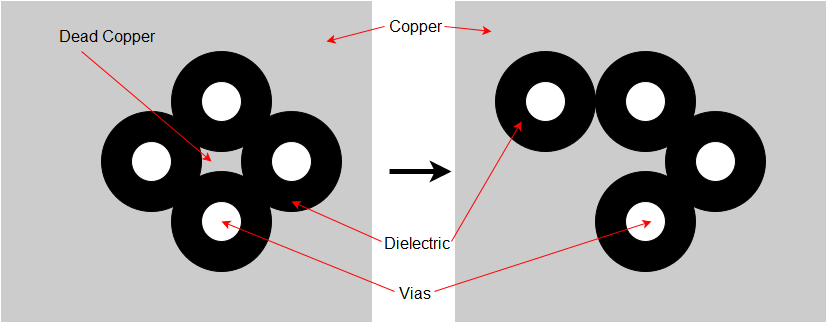
\includegraphics[scale = 0.4]{images/Dead_Copper.png}
\caption{Dead Copper. To the right, dead copper is avoided by moving one via.}
\label{fig:Dead copper}
\end{figure}

\subsection{Possible Routing Improvement}
The auto router caused some wires to make long detours.
Manual routing of some signals could've shortened these distance, but was not critical to the design.
Wires in the same parallell buses should ideally have equal lengths, to ensure all signals in are synchronized.
Some wires in the \gls{ebi} bus, and the bus between the \gls{fpga} and the frame buffer, had varying lengths - potentially create race conditions.
No anomalies were discovered, and the team assumed it was not a problem.
However, modern general purpose computers should be careful to avoid these race conditions \cite{race-conditions}.

\subsection{Bad Soldering}
Some issues arised because of components not being properly soldered onto the \gls{pcb}. Examples are component pins with partial or no contact to the \gls{pcb}, and pins touching several footprint connectors.

\subsubsection{Partially Soldered Voltage Regulator}
It was critical to verify that the power planes worked, as the computer would be dead without power.
Every necessary part that delivered power was soldered on, including power headers and the 3.3 voltage regulator.
External power was run through the power headers.
Measuring different places with a multimeter, anomalies were discovered.
The voltmeter showed only 2.3V, instead of 3.3V.
Further testing revealed that one of the voltage regulator pins hadn't been soldered properly, resulting in a loss of 1V.
Fixing this, the digital \(V_{CC}\) plane contained the correct 3.3V.

\subsection{Incorrect Wiring}
Most \gls{pcb} problems were due to incorrect wiring.
Either signals were having unexpected values, short-circuits had occurred, or other unexpected behaviour.
In the next sections, the most significant wiring issues are addressed and how they were fixed.

\subsubsection{Short-circuits in Buttons}
The group discovered that the buttons were wired wrong, since they caused short-circuits.
The reason was sloppy study of the datasheet, as shown in figure \ref{fig:Button Issue}.
Luckily, this could be remedied by rotating the button 90 degrees, if adjusting the physical connectors to fit the footprint.

\begin{figure}[h!]
\centering
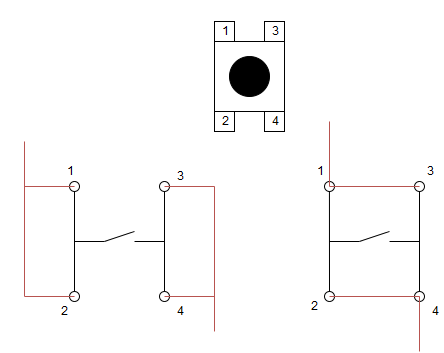
\includegraphics[scale=0.5]{images/Button_Issue.png}
\caption{Top figure shows the button as it looks like on the \gls{pcb}. On the left: Correct wiring according to datasheet. On the right: Incorrect wiring leading to short-circuit}
\label{fig:Button Issue}
\end{figure}

\subsubsection{No Output from Oscillators}
Testing the oscillators, they did not seem to work.
The datasheet for these components clearly stated that connecting the E/D pin to either 'No Connect' or '1' equaled active, so the team did not connect it.
When E/D was connected to \(V_{CC}\), the problem was solved.

\subsubsection{Incorrect Power Supply to Vref and DACs}
The Vref chip was supplied with 3.3V, but should have been supplied with analogue 5V instead.
This could be remedied by cutting on the 3.3V power trace, since the trace is located on the top layer and no other traces are beneath it.
The analogue 5V could then be connected via header from the voltage regulator to the input pin on the Vref chip.
\newline
The DACs were supplied with analogue 5V, but should have been supplied with 3.3V; the analogue 5V should go to the Vref chip instead.
This was solved by switching the two connections.

\subsubsection{Faulty Connected BNCs}
The \gls{bnc} connections were faulty wired.
Each \gls{bnc} had two connections, excluding the socket itself, connected to the \gls{bnc} cable.
One of these would go to ground, while the other would receive the signal destined for the oscilloscope, but these connections was switched.
The group fixed this by running wires to the correct connections.

\subsubsection{FPGA Configuration Issue}
When the \gls{fpga} would complete configuration, it was supposed to set a signal high, which was connected to the \gls{mcu}, saying it was ready. ¨
However, the \gls{mcu} seemed to ignore this signal.
What caused this problem was too hasty study of the manual describing configuration of the \gls{fpga}.
An unnecessary connection to \(V_{CC}\) forced the Done signal into the \gls{mcu} to always be high, even when the \gls{fpga} was not configured.
Since the \(V_{CC}\) connection couldn't be removed, a workaround had to be devised.

By introducing a transistor, and making the signal active low on the \gls{mcu} side, the group managed to make the \gls{mcu} notice when configuration was complete.
The problem and solution is shown in detail in figure \ref{fig:Done Issue}.
This solution was possible because the wire went through the \gls{jtag} header.

\begin{figure}[h!]
\centering
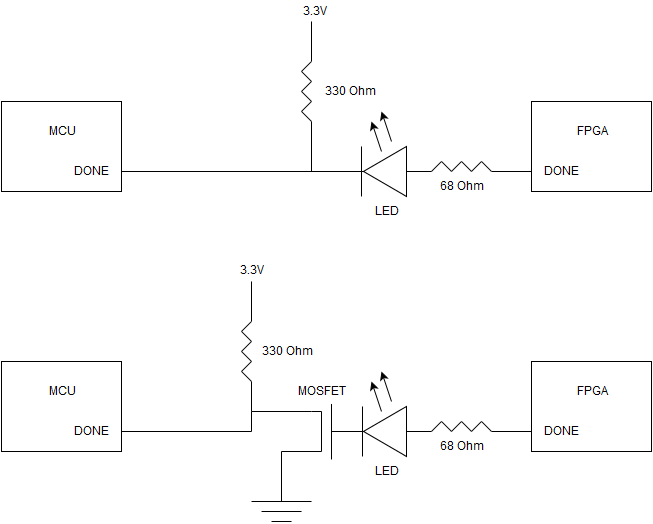
\includegraphics[scale=0.5]{images/Done_Signal_Issue.png}
\caption{Problem and solution of Done signal
         \newline
         Top: Done signal into \gls{mcu} was always logical high
         \newline
         Bottom: Done signal into \gls{mcu} was now active low. The transistor was activated when the configuration was complete, forcing the 3.3V to ground}
\label{fig:Done Issue}
\end{figure}

After further studying of the \gls{fpga} configuration manual \cite[page 42]{fpga-configuration},
it was discovered that the manual was different from what was intended in the group's design,
so there was need for an extra \(V_{CC}\) connection.

\subsubsection{Noise Reduction}
The diode which was intended to reduce noise in the analogue plane, had no noticable effect.
The reason was probably focus on the current leakage, and not noise itself.
The team solved this using a ferrite bead instead of the diode.
A ferrite bead is a component designed to suppress high-frequency noise.

Noise was reduced, but the ferrite bead itself worked also as a resistor, allowing only a small current flow through.
Connecting a resistor with very low resistance (15 Ohm) in parallell with the ferrite bead, current was able to flow freely through this connection.

\subsection{PCB Placement and Footprints}
It would have been beneficial to place the 3.3V voltage regulator closer to the \gls{jtag} debugging port, since the Xilinx \gls{jtag} platform cable required a 3.3V power supply.

The micro \gls{usb} footprint originally contained mounting holes, but were for some reason never drilled during manufacturing.
Luckily, these did not act as connectors, and the team could therefore solder the \gls{usb} receptacle onto the \gls{pcb} like a surface mounted component.

\subsection{Component sizes}
In hindsight, it would have been better to order bigger components.
Since this was a prototype board with mostly hand-soldering, an increase in size would only be beneficial.
Should the project should go into large scale production, the size could have been reduced.


\section{Component Ordering}
The group feels they could've been more thorough with datasheet inspection before finalising component orders.
While waiting for the first delivery, it was discovered that the ordered \gls{led}s were reverse mounted, and not compatible with the \gls{pcb}.
Hence, a new set of \gls{led}s with the correct footprint were ordered.
While this was a cheap component, it could very well have been an important component, resulting in unnecessary delays and waste of money.

Several \gls{dac}s were destroyed, caused by short-circuits during testing.
This resulted in a shortage of \gls{dac}s, which were essential for the design.
For future reference a surplus of fragile components should be ordered.

\section{Oscillator}
To acheive a high clock frequency on the \gls{fpga}, a 100 MHz oscillator was added to the board.
Using it as the main clock signal, the \gls{fpga} was not able to produce correct output.
An oscilloscope was used to measure the oscillator output on a header.
If a hand was placed in close proximity of the board, the oscillator signal was significantly affected.
This problem was solved by using the 48 MHz oscillator instead.

\section{Drawing Artefacts}
\label{discussion:artefacts}
The drawing artefacts explained in Section \ref{results:artefacts} are possible to remove.
If a third input value for intensity were to be added, one could turn the electron beam off when moving the beam between primitives.

The other artefact mentioned, the dotted lines, could be removed by adding analogue circuitry between the \gls{dac} output and the BNC connectors.
It is possible to slew the electron beam from one point to the next, using analogue integration, to archive a smooth transition between points.
An example of such circuitry has been implemented in the 80's in a similar project \cite{vector-graphic-crt}.

If \vthreek were to support an intensity value in addition to x and y, the architecture and \gls{pcb} would require changes.

\section{Improvements}
Further improvements - which ultimately were not implemented due to time constraints or complexity - were discussed by the group and are detailed here.

The auto router caused some wires to make long detours.
More manual routing of signals could've generally shortened these distances.
Wires in the same parallel buses should ideally have equal lengths, to ensure all signals in it are synchronized. 
Failure to do so could result in race conditions \cite{race-conditions}. 
This was not critical, and was thus not implemented.

Before any actual coding and soldering, the group spent some time planning the architecture.
It was argued that implementing floating point would better conform to the industry standards of representing and processing vector graphics, and that it would offer more precise calculations.

The final implementation of the processor is a multi-cycle RISC/MIPS inspired processor.
In this design, one instruction is executed each for second or third clock cycle.
To increase the number of instructions per cycle, the processor could have been pipelined.
Given the time constraint, the group never found the time to implement a pipelined processor.

The processor could also have been made into a SIMD-like, multi-core processor, which would further improve the performance.
This would allow for greater efficiency when performing modifications to batches of primitives.

Interactivity between the user and the graphics could have been implemented, using the included buttons and joystick. A game was discussed as a possible demo, but was deemed to complex and time demanding, given that other parts of the system were more critical to implement.

A toolchain with a higher level language was not prioritised high enough to be done anything with.

The \gls{isa} could have been extended, i.e. with convenient operations that would shorten the program length and solve unintuitive syntax.
